\documentclass[12pt]{article}
%\documentclass{nature}

% Including pdf figures
\usepackage{graphicx}
\graphicspath{ {../Plots/} }
\usepackage{pdfpages}
\usepackage{epstopdf}
\epstopdfsetup{outdir=./}
%really place a figure in a location
\usepackage{float}
%Overrun caption
\usepackage[CaptionAfterwards]{fltpage}
% Math stuff
\usepackage{amsmath}
\usepackage{stix}
% Bibliographies
\usepackage[numbers]{natbib}
\bibpunct{(}{)}{,}{a}{}{;} 

\usepackage[flushleft]{threeparttable}

\usepackage[font={scriptsize}]{caption}

\usepackage{lineno} %gives line numbers with \lineno command

\usepackage{setspace}
\onehalfspace

\usepackage{tikz}%for putting words on figures
\usetikzlibrary{positioning}%for relative positioning

%to rotate figures
\usepackage{rotating}
\usepackage{pdflscape}

\begin{document}

\section*{Figures}

\begin{figure}[!h]
\centering
\centerline{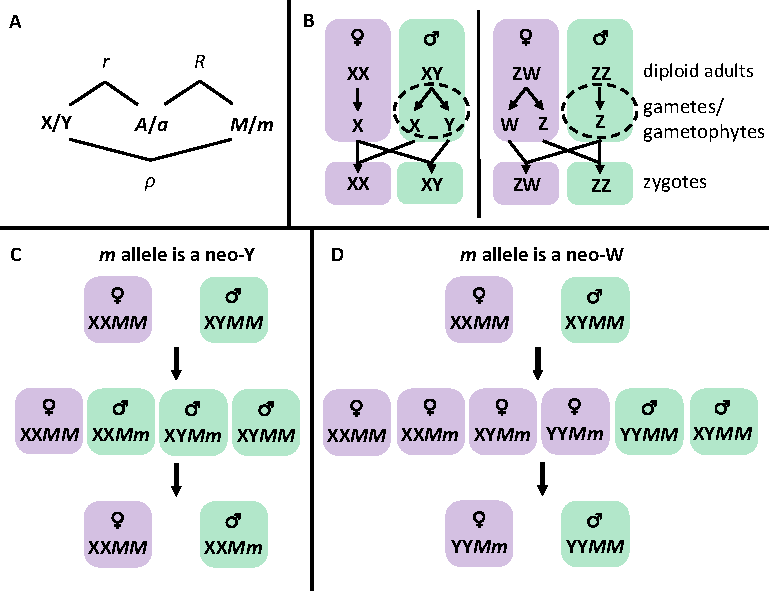
\includegraphics[width=\linewidth]{Sex_determination_outline.pdf}}
\caption{}
\end{figure}

\begin{figure}[!h]
\centering
\centerline{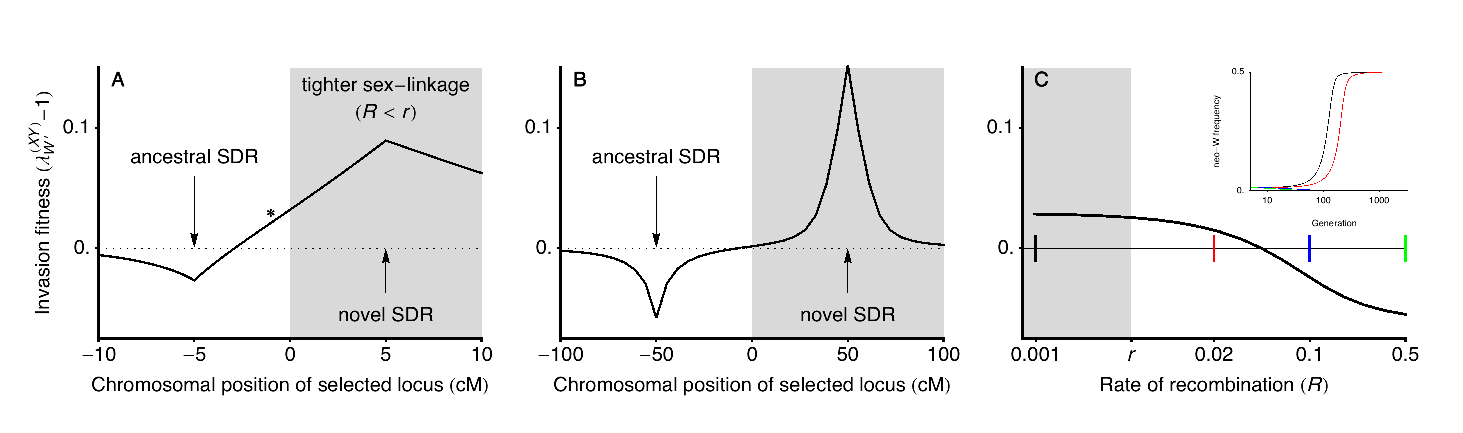
\includegraphics[width=\linewidth]{PositionPlot_SexAntagTighter.eps}}
\caption{}
\end{figure}

\begin{figure}[!h]
\centering
\centerline{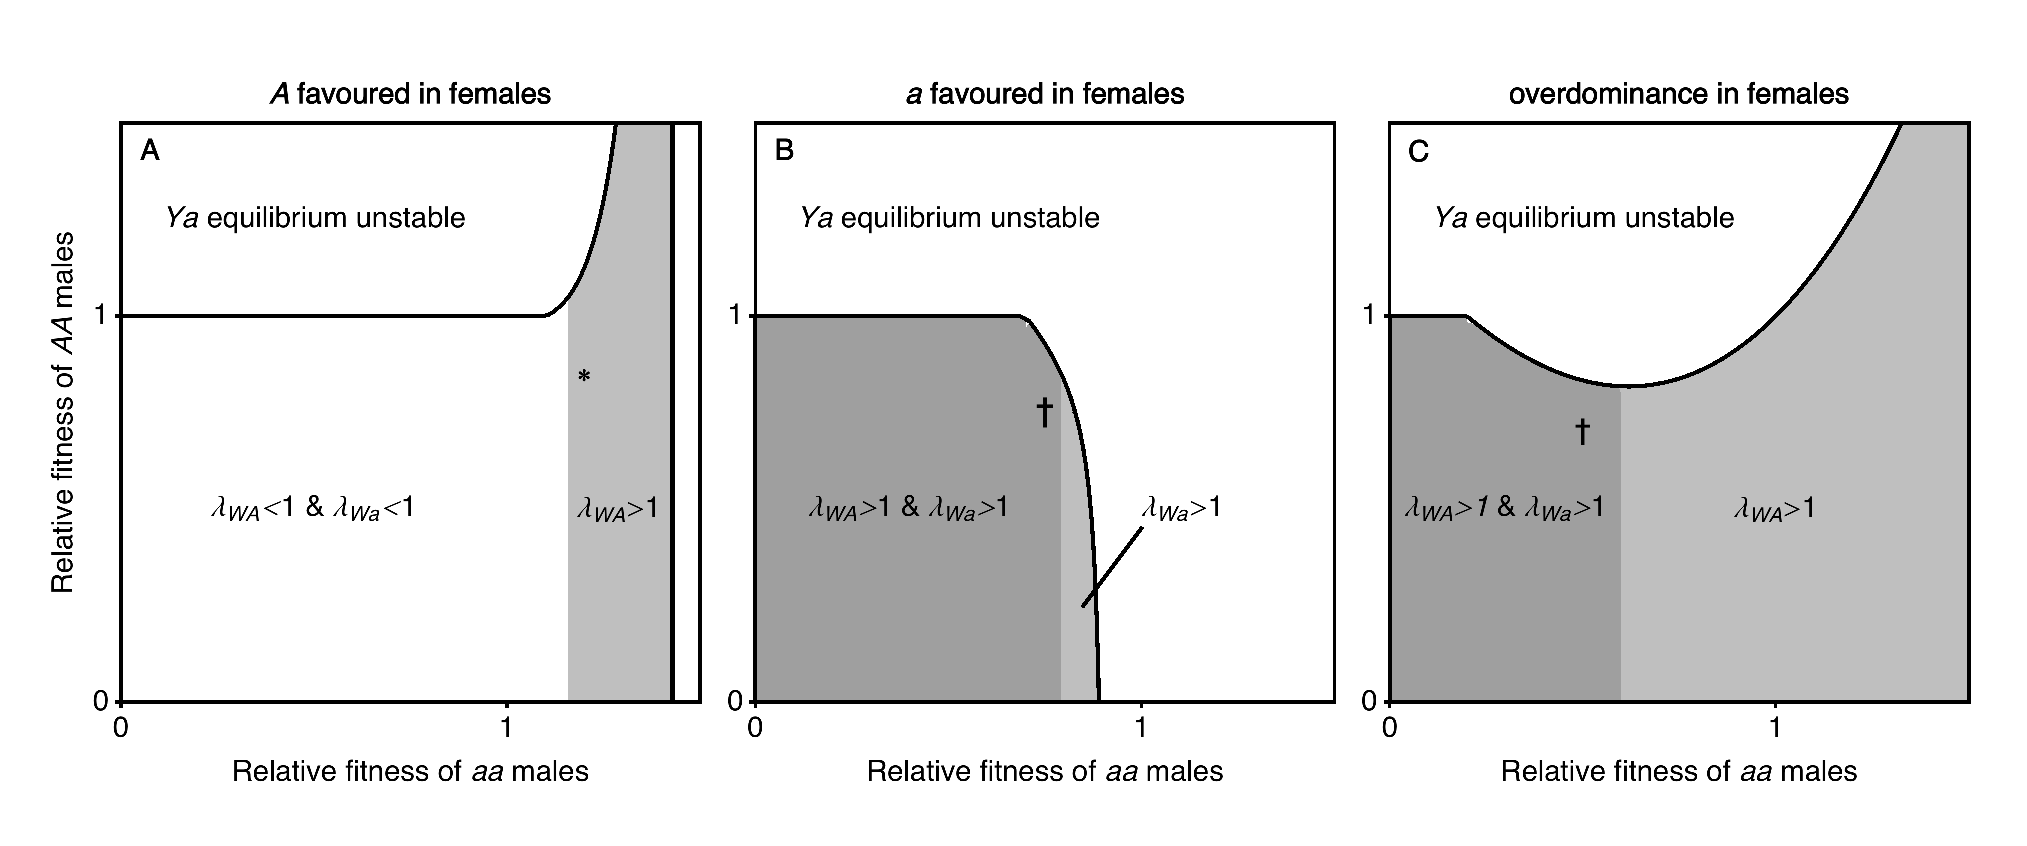
\includegraphics[width=\linewidth]{Region_plot_combined.eps}}
\caption{}
\end{figure}

\newpage
\begin{figure}[!h]
\centering
\centerline{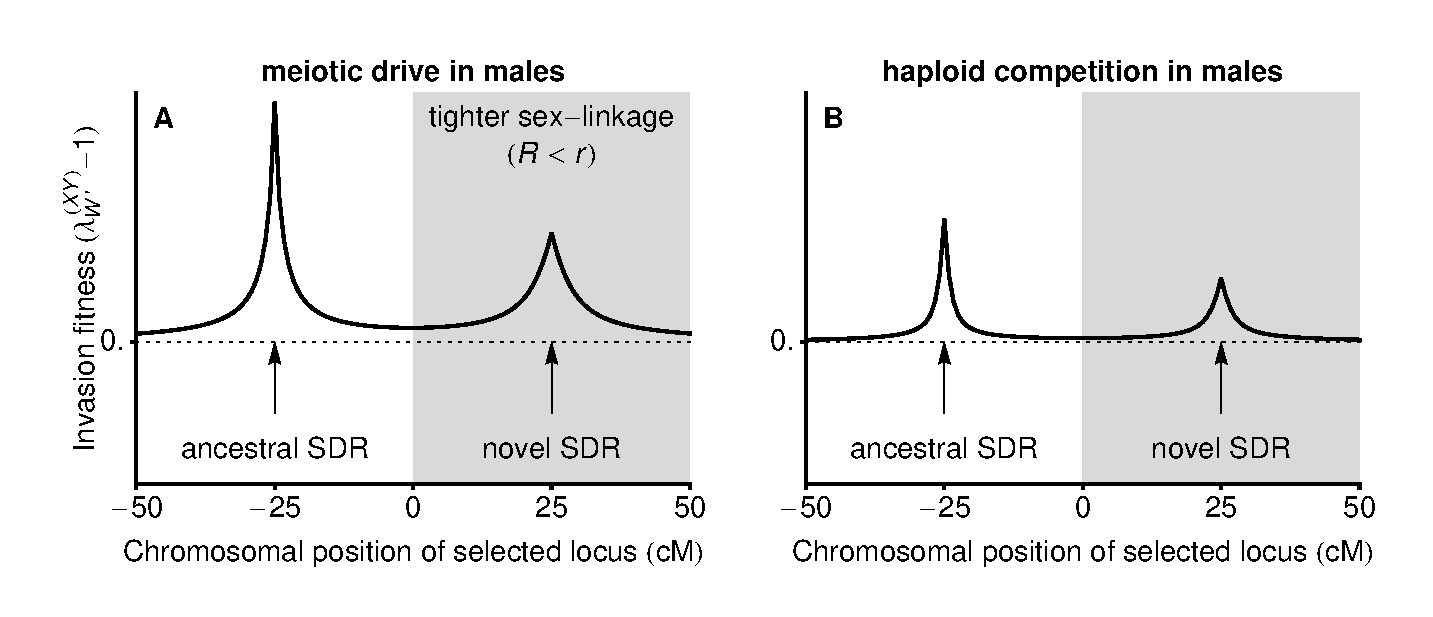
\includegraphics[width=\linewidth]{PositionPlot.eps}}
\caption{}
\end{figure}

\begin{figure}[!h]
\centering
\centerline{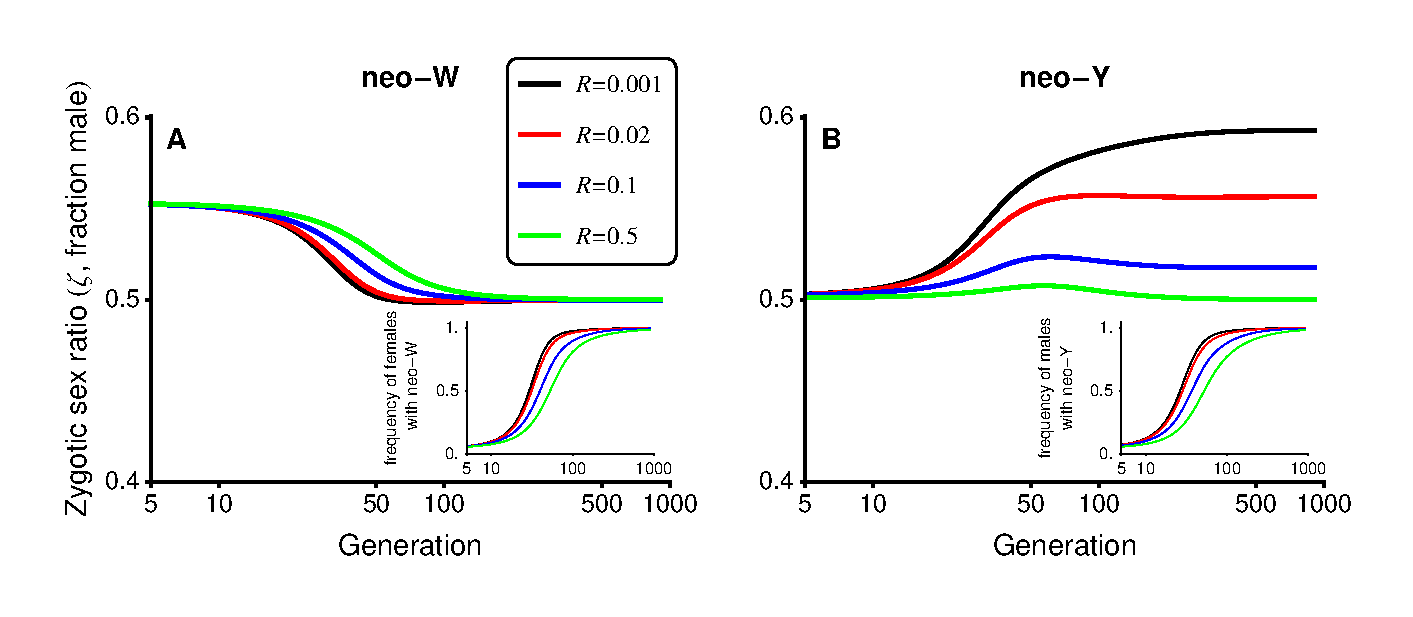
\includegraphics[width=\linewidth]{Temporal_SR.eps}}
\caption{}
\end{figure}

\end{document}



